\documentclass{IEEEtran}

\usepackage{cite}
\usepackage{amsmath}
\usepackage{amsfonts}
\usepackage{bm}
\usepackage{algorithm}
\usepackage{algorithmic}
\usepackage{booktabs}
\usepackage{multirow}

\usepackage{graphicx}
\usepackage{subfig}

\usepackage{xeCJK}

\usepackage{fontspec}
\setmainfont{Times New Roman}

\setCJKfamilyfont{song}{SimSun}
\newcommand{\song}{\CJKfamily{song}}

\setCJKfamilyfont{kai}{KaiTi}
\newcommand{\kai}{\CJKfamily{kai}}




\begin{document}

\title{A fast and efficient multi-objective optimization algorithm}
\author{Dawei Zhan}
\maketitle

\begin{abstract}
NSGA-II is very popular for solving multi-objective optimization problems. But its efficiency  decreases gradually as the number of variables increases. In this work, we propose a novel multi-objective optimization algorithm to solve this problem. Numerical experiments show that our algorithm performs significantly better than NSGA-II on the test problems.
\end{abstract}




\section{Introduction}
\label{section_introduction}

\song 这是中文 \kai 这是楷体,目标函数$f(\bm{x})$其中$\bm{x}$是设计变量。

NSGA-II~\cite{Deb_2002} is very popular for solving multi-objective optimization problems. Popular algorithms for multi-objective optimization problems are~\cite{Deb_2002,Zhang_2007,Deb_2014}.


Section~\ref{section_introduction} gives the introduction. Section~\ref{section_background} introduces the backgrounds of this work.



\section{Backgrounds}
\label{section_background}

We have a scalar $x$, a vector $\bm{x}$, a random variable $X$, a matrix $\bm{X}$, where $\bm{x} = [x_1,x_2,\cdots,x_d]$, $\bm{X} = \{\bm{x}^{(1)},\bm{x}^{(2)},\cdots,\bm{x}^{(n)}\}$, where n $n$ is the number of points.

we try to solve the following optimization problem in (\ref{eq_1}).

\begin{equation}
\label{eq_1}
	\text{minimize}~ f(\bm{x})
\end{equation}



The algorithm is given in Algorithm~\ref{alg_1}.

\begin{algorithm}
	\caption{Algorithm of computing the maximum of two variables}
	\label{alg_1}
	\begin{algorithmic}
		\REQUIRE $a$, $b$
		\ENSURE $c = \max(a,b)$
		\IF{$a>b$}
		\STATE $c=a$
		\ELSE 
		\STATE $c=b$
		\ENDIF 
	\end{algorithmic}
\end{algorithm}




\begin{enumerate}
	\item Step 1: see whether $a$ is greater than $b$.
	\item Step 2: if it is true, return $a$.
	\item Step 3: if not, return $b$.
\end{enumerate}









\subsection{Multi-objective optimization problem}




\subsection{NSGA-II}



\subsubsection{Non-dominated Sorting}

\subsubsection{Crowding Distance}


\section{Proposed Algorithm}

\section{Numerical Experiments}


The experiment results are given in Table~\ref{table_1}.

\begin{table}
	\centering
	\caption{Results of NSGA-II and X}
	\label{table_1}
	\begin{tabular}{c c c}
		\toprule
		problem & NSGA-II & X \\
		\midrule
		$f_1$ &  7.8 (6.1) & 10.8 (5.4) \\
		$f_2$ &  8.9 (7.2) & 11.9 (6.5) \\
		$f_3$ &  9.0 (8.3) & 12.0 (6.6) \\
		\bottomrule 
	\end{tabular}
\end{table}



\begin{table}
	\centering
	\caption{Results of NSGA-II and X}
	\label{table_2}
	\begin{tabular}{c c c c c}
		\toprule
		\multirow{2}{*}{problem} & \multicolumn{2}{c}{NSGA-II} & \multicolumn{2}{c}{X}\\
		        & mean  & std & mean & std \\		
		\midrule
		$f_1$ &  7.8 & (6.1) & 10.8 & (5.4) \\
		$f_2$ &  8.9 & (7.2) & 11.9 & (6.5) \\
		$f_3$ &  9.0 & (8.3) & 12.0 & (6.6) \\
		\bottomrule 
	\end{tabular}
\end{table}



The convergence curves are given in Figure~\ref{fig_1}.

\begin{figure}
	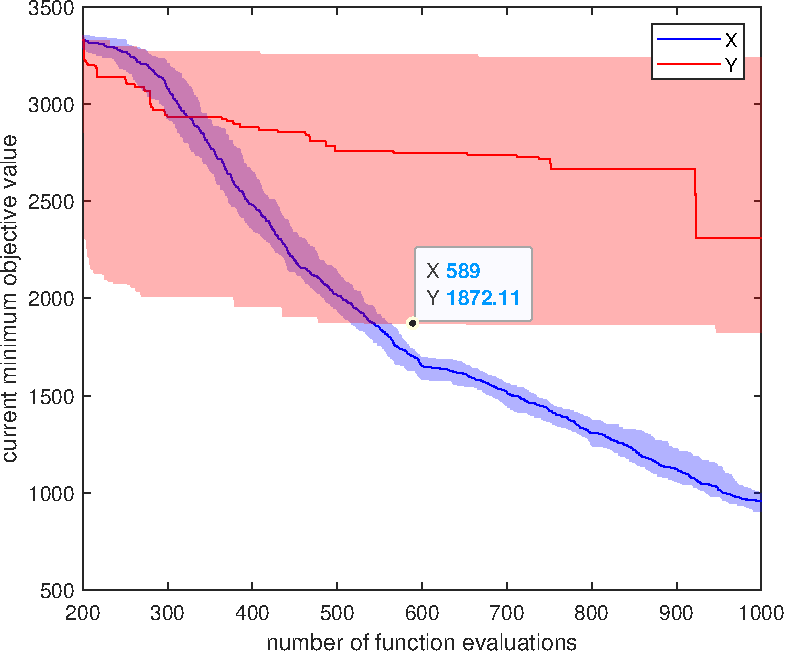
\includegraphics[width=\linewidth]{figure_1.pdf}
	\caption{Convergence curves}
	\label{fig_1}
\end{figure}






\begin{figure*}
	\centering
	\subfloat[$f_1$]{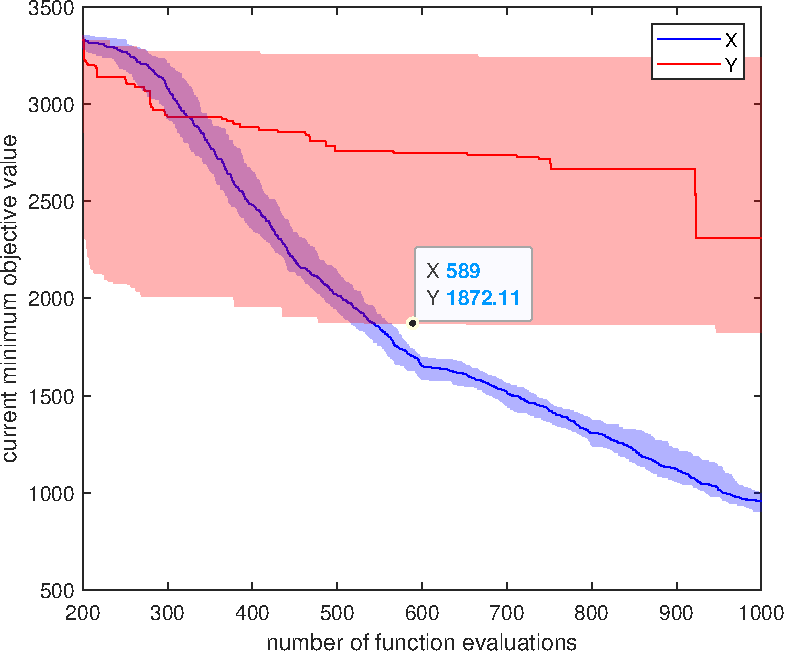
\includegraphics[width=0.3\linewidth]{figure_1.pdf}} \hfil
	\subfloat[$f_2$]{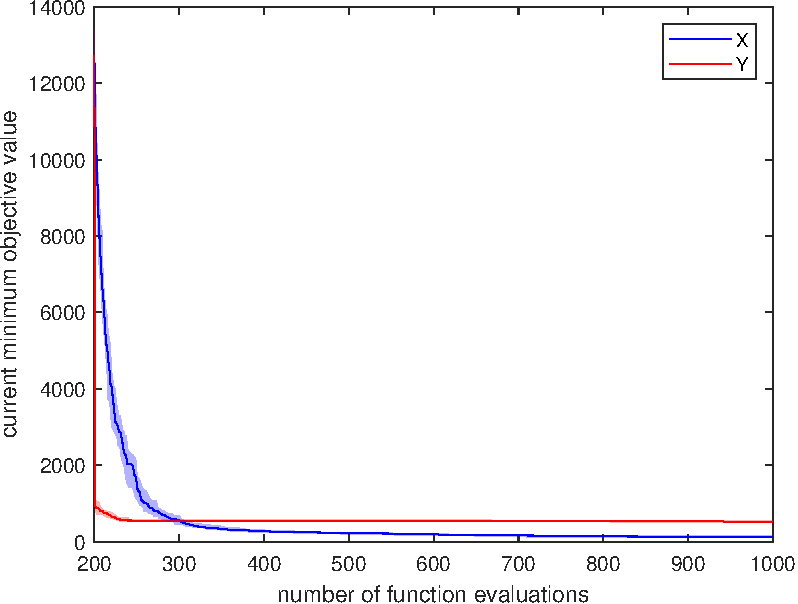
\includegraphics[width=0.3\linewidth]{figure_2.pdf}} \\
	\subfloat[$f_3$]{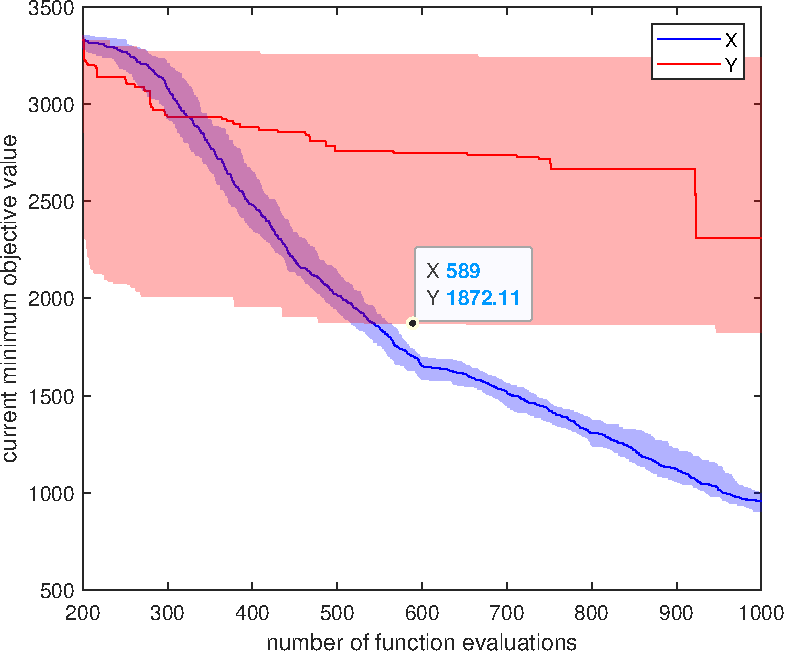
\includegraphics[width=0.3\linewidth]{figure_1.pdf}} \hfil
	\subfloat[$f_4$]{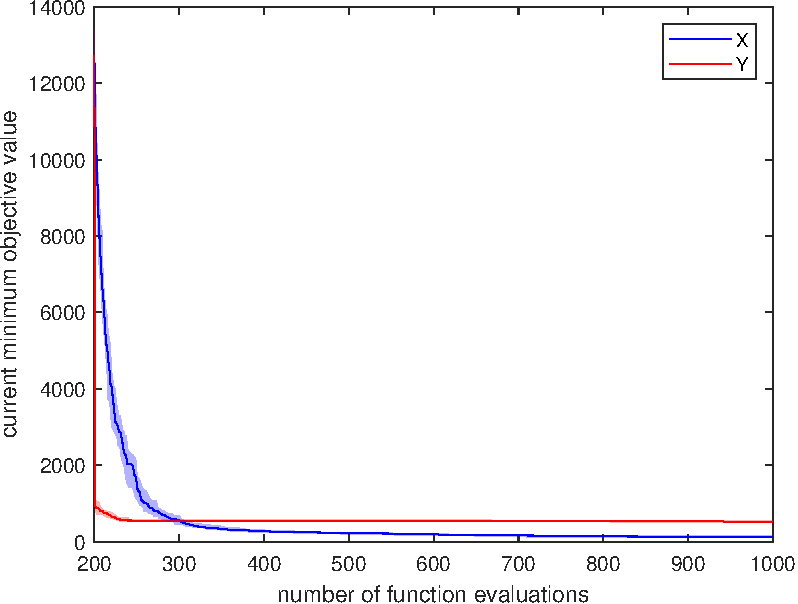
\includegraphics[width=0.3\linewidth]{figure_2.pdf}} 
	\caption{Convergence curves}
	\label{fig_2}
\end{figure*}







\section{Conclusion}





\bibliographystyle{IEEEtran}
\bibliography{my_ref.bib}
	
	
	
	
	
	
	
\end{document}